\documentclass[a4paper,12pt]{article}

%%% Работа с русским языком
\usepackage{cmap}					% поиск в PDF
\usepackage{mathtext} 				% русские буквы в формулах
\usepackage[T2A]{fontenc}			% кодировка
\usepackage[utf8]{inputenc}			% кодировка исходного текста
\usepackage[english,russian]{babel}	% локализация и переносы

%%% Дополнительная работа с математикой
\usepackage{amsmath,amsfonts,amssymb,amsthm,mathtools} % AMS
\usepackage{icomma} % "Умная" запятая: $0,2$ --- число, $0, 2$ --- перечисление

%% Номера формул
%\mathtoolsset{showonlyrefs=true} % Показывать номера только у тех формул, на которые есть \eqref{} в тексте.
%\usepackage{leqno} % Нумерация формул слева

%% Свои команды
\DeclareMathOperator{\sgn}{\mathop{sgn}}

%% Перенос знаков в формулах (по Львовскому)
\newcommand*{\hm}[1]{#1\nobreak\discretionary{}
{\hbox{$\mathsurround=0pt #1$}}{}}

%%% Работа с картинками
\usepackage{graphicx}  % Для вставки рисунков
\graphicspath{{Materials/}{images2/}}  % папки с картинками
\setlength\fboxsep{3pt} % Отступ рамки \fbox{} от рисунка
\setlength\fboxrule{1pt} % Толщина линий рамки \fbox{}
\usepackage{wrapfig} % Обтекание рисунков текстом
\usepackage{floatrow}

%%% Работа с таблицами
\usepackage{array,tabularx,tabulary,booktabs} % Дополнительная работа с таблицами
\usepackage{longtable}  % Длинные таблицы
\usepackage{multirow} % Слияние строк в таблице

%%% Теоремы
\theoremstyle{plain} % Это стиль по умолчанию, его можно не переопределять.
\newtheorem{theorem}{Теорема}[section]
\newtheorem{proposition}[theorem]{Утверждение}
 
\theoremstyle{definition} % "Определение"
\newtheorem{corollary}{Следствие}[theorem]
\newtheorem{problem}{Задача}[section]
 
\theoremstyle{remark} % "Примечание"
\newtheorem*{nonum}{Решение}

%%% Программирование
\usepackage{etoolbox} % логические операторы

%%% Страница
%\usepackage{extsizes} % Возможность сделать 14-й шрифт
\usepackage{geometry} % Простой способ задавать поля
	\geometry{top=30mm}
	\geometry{bottom=30mm}
	\geometry{left=10mm}
	\geometry{right=10mm}
 %

\usepackage{setspace} % Интерлиньяж
%\onehalfspacing % Интерлиньяж 1.5
%\doublespacing % Интерлиньяж 2
%\singlespacing % Интерлиньяж 1

\usepackage{lastpage} % Узнать, сколько всего страниц в документе.

\usepackage{soulutf8} % Модификаторы начертания

\usepackage{hyperref}
\usepackage[usenames,dvipsnames,svgnames,table,rgb]{xcolor}
\hypersetup{				% Гиперссылки
    unicode=true,           % русские буквы в раздела PDF
    pdftitle={Заголовок},   % Заголовок
    pdfauthor={Автор},      % Автор
    pdfsubject={Тема},      % Тема
    pdfcreator={Создатель}, % Создатель
    pdfproducer={Производитель}, % Производитель
    pdfkeywords={keyword1} {key2} {key3}, % Ключевые слова
    colorlinks=true,       	% false: ссылки в рамках; true: цветные ссылки
    linkcolor=red,          % внутренние ссылки
    citecolor=green,        % на библиографию
    filecolor=magenta,      % на файлы
    urlcolor=cyan           % на URL
}

%\renewcommand{\familydefault}{\sfdefault} % Начертание шрифта

\usepackage{multicol} % Несколько колонок

% Мои "дополнительные" пакеты
\usepackage{textcase} 
\usepackage{pdfpages}
\usepackage{amsmath}


\author{Дмитрий Павлов}
\title{Студент 1 курса ФИВТ МФТИ}
\date{\today}

\begin{document} % конец преамбулы, начало документа

\thispagestyle{empty}
\begin{center}
	\vspace{0.5ex}
	
	\textbf{ \\ \MakeTextUppercase{<<Московский Физико-технический институт>>}}
\end{center}
\vspace{13ex}
\begin{flushright}
	\noindent
	{Дмитрий Павлов}
	\\
	\textit{Студент факультета инноваций\\ и высоких технологий\\(группа 790)}
\end{flushright}
\begin{center}
	\vspace{23ex}
	{\LARGE\textbf{Лабораторная работа №2.2.1}}
	\vspace{1ex}
		
	\textbf{\large{<<Исследование взаимной диффузии газов>>}}
	
	\vfill
	Долгопрудный 
	
	{\today}
\end{center}

\newpage
%------------------------------------------------------------------------
\subsection{Цель работы:} 
\begin{itemize}
    \item
    Регистрация зависимости концентрации гелия в воздухе от времени с помощью датчиков теплопроводности при разных начальных давлениях смеси газов.
    
    \item
    Определение коэффициента диффузии по результатам измерений.
\end{itemize} 

\subsection{В работе используются:} 
\begin{itemize}
    \item
    измерительная установка; 
    
    \item
    форвакуумный насос;
    
    \item
    баллон с газом (гелий);
    
    \item
    источник питания;
    
    \item
    магазин сопротивлений;
    
    \item
    манометр;
    
    \item
    секундометр.
\end{itemize}     

\section{Теоретический материал:}
    \textit{Диффузией} называется самопроизвольное перемешивание молекул,         происходящее вследствие их теплового движения. В тех случаях, когда происходит перемешивание молекул одного вещества, говорят о \textit{самодиффузии}, а если перемешиваются разные молекулы -- о \textit{взаимной} (или \textit{концентрационной}) диффузии.

    Рассмотрим процесс выравнивания концентраций двух различных газов. Пусть концетрации одного из компонентов смеси в сосудах $V_1$ и $V_2$ равны $n_1$ и $n_2$ соответственно. Плотность диффузионного потока (количество вещества, проходящее в единицу времени через единичную поверхность) определяется законом Фика:
    
    \begin{equation}
        j = -D\dfrac{\partial n}{\partial x},
    \end{equation}
    
    где $D$ -- коэффициент взаимной диффузии газов,  a $j$ -- плотность потока частиц.
    
    В условиях установки, приведенной на рис.1, объем соединительной трубки длиной $l$ и площадью $S$ мал по сравнению с объемами сосудов и концентрацию газов можно считать постоянной внутри каждого сосуда. Поэтому величина $J = jS = -DS(\partial n / \partial x)$ не меняется вдоль трубки. Отсюда получаем, что
    
    \begin{equation}
        J = -DS\dfrac{n_1 - n_2}{l}
    \end{equation}
    
    Из закона сохранения вещества в любой момент времени $V_1n_1 + V_2n_2 = const$, отсюда, обозначив за $\Delta n_1$ и $\Delta n_2$ изменения концентраций в объемах $V_1$ и $V_2$ за время $\Delta t$, имеем
    
    \begin{equation}
        V_1 \Delta n_1 = -V_2 \Delta n_2 = J \Delta t = -DS\dfrac{n_1 - n_2}{l} \Delta t
    \end{equation}
    
    Путем математических преобразований (разделим обе части на $\Delta t$, первое -- на $V_1$, второе на $V_2$ и вычитая), найдем
    
    \begin{equation}
        \dfrac{d(n_1 - n_2)}{dt} = \dfrac{dn_1}{dt} - \dfrac{dn_2}{dt} = -\dfrac{n_1 - n_2}{l}DS(\dfrac{1}{V_1} + \dfrac{1}{V_2})
    \end{equation} 
    
    Интегрируя (4), получим зависимость разности концентраций от времени:
    
    \begin{equation}
        n_1 - n_2 = (n_1 - n_2)_0\exp(-t/\tau),
    \end{equation}
    
    где $n_1 - n_2)_0$ -- разность концентрация в начальный момент времени,
    $\tau = \dfrac{V_1V_2}{V_1 + V_2}\dfrac{l}{SD}$ -- характерное время, определяемое параметрами установки и величиной коэффициента диффузии.

    Для измерения концентраций в данной установке используется зависимость теплопроводности газовой смеси от ее состава. Тонкая проволока радиуса $r$, натянутая вдоль оси цилиндра радиуса $R$, нагревается электрическим током. Вследствие теплопроводности газа происходит теплопередача от проволоки к стенкам. При этом количество теплоты, переданное в единицу времени, равно
    
    \begin{equation}
        Q = \varkappa\dfrac{2\pi L}{\ln(R/r)}(T_1 - T_2)
    \end{equation}
    
    Измерение разности концентраций производится с помощью мостовой схемы (см. рис.2). При достаточно малых изменениях концентраций величина тока, проходящая через гальванометр, пропорциональна разности концентраций. Поэтому показания гальванометра во времени будут изменяться по тому же закону, что и разность концентраций, т.е.
    
    \begin{equation}
        N = N_0\exp(-t/\tau),
    \end{equation}
    
    где  $N_0$ -- показания в начальный момент времени.

\newpage

\section{Экспериментальная установка:}

    \begin{center}
        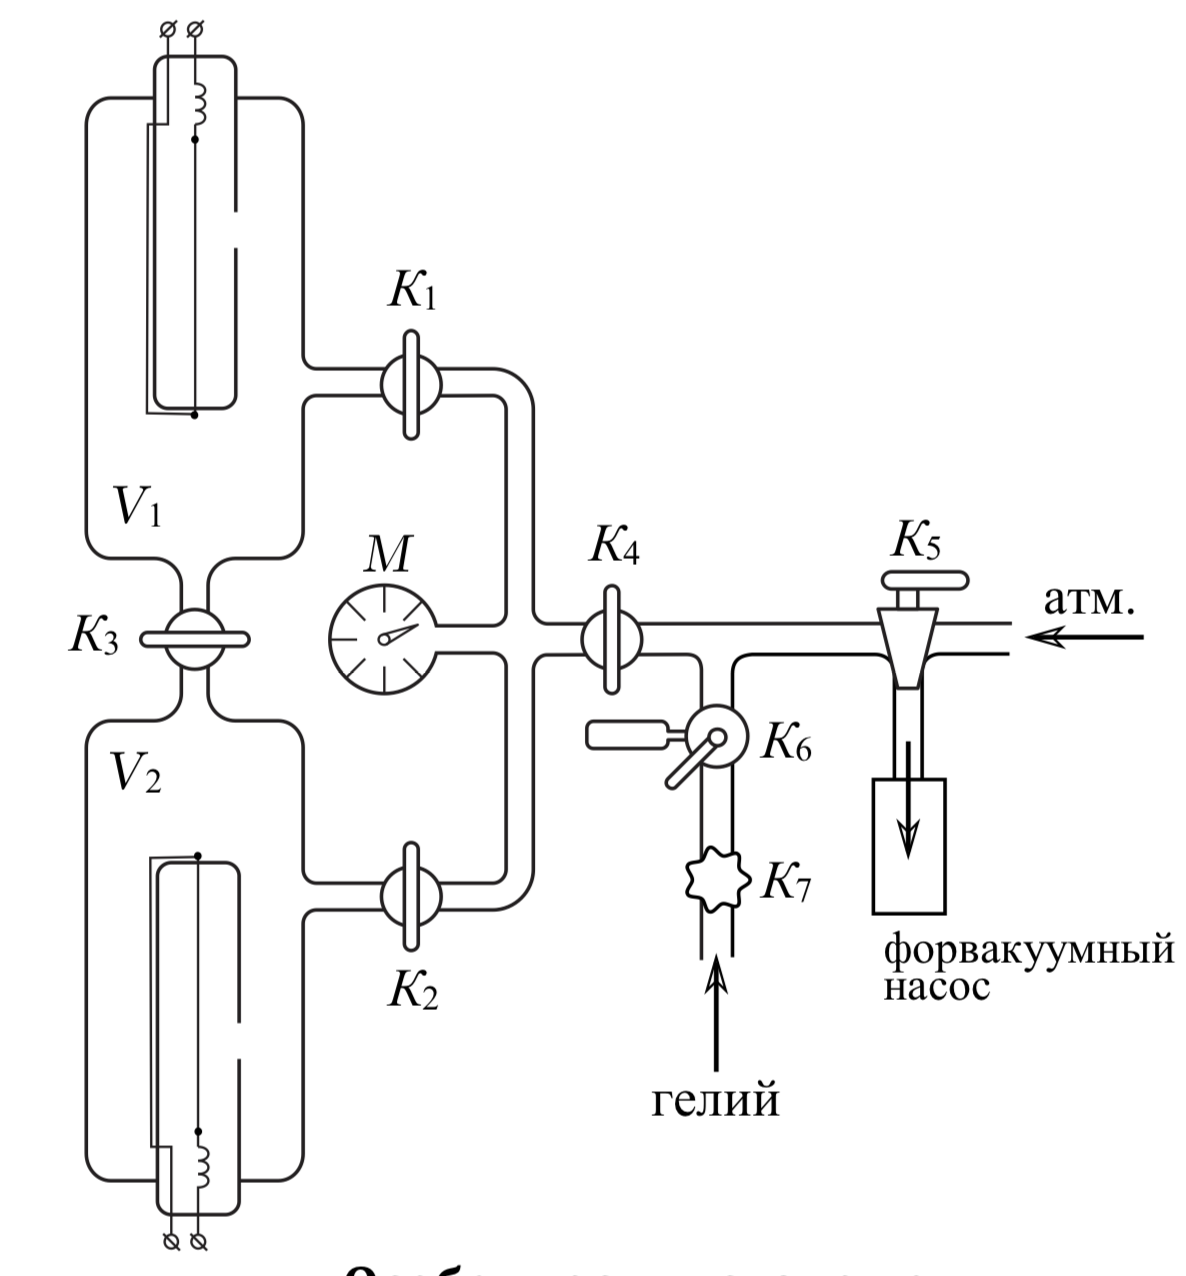
\includegraphics[scale = 0.4]{scheme.png}    
        
        Схема установки.
    \end{center}
    
    Общая схема установки представлена на рис.1. (вариант А). 
    Установка состоит из двух сосудов объемами $V_1$ и $V_2$, соединенных краном К3, форвакуумного насоса, манометра М и системы напуска гелия (краны К6 и К7). Кран К5 служит для подключения форвакуумного насоса к установке, подачи воздуха в установку и соединения форвакуумного насоса с атмосферой. Сосуды можно соединять как с форвакуумным насосом, так и с системой напуска гелия. Манометр регистрирует давление газа, до которого заполняют сосуд.
    
    \begin{center}
	    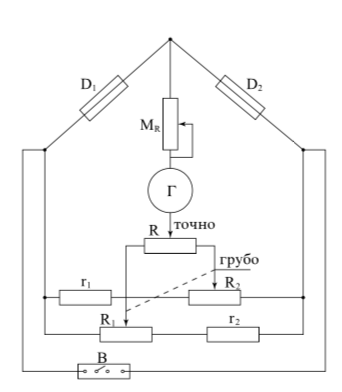
\includegraphics[scale = 1]{scheme2.png}
	    
        Схема мостового соединения
    \end{center}
    
    На рис.2. приведена схема электрического соединения. $D_1$ и $D_2$ -- сопротивления проволок датчиков парциального давления, которые составляют одно плечо моста.  Второе плечо моста составляют сопротивления $R_1, R_2 (R_1 \gg r_1, R_2 \gg r_2)$, служащие для грубой регулировки моста. Точная регулировка моста достигается с помощью потенциометра R.
    
\newpage
\section{Выполнение работы:}
    \subsection{Установка и внешние условия:}
    
        Параметры установки:
        \begin{center}
            $V_1  = V_2 = 1200 $ см$^3$ , $\frac{L}{S} = 5.5$см$^{-1}$    
        \end{center}
        Атмосферное давление:
        \begin{center}
            $P_\textit{атм} =  98156 \hspace{3pt} \textsf{Па} $    
        \end{center}
    
    \subsection{Запуск установки:}
    
        Откачаем установку до давления $\sim 0.1 \textsf{ Торр}$ и проведем калибровку моста (показания вольтметра должны быть близки к нулевой отметке). 
    
        Приготовим рабочие смеси. Для этого откачаем всю установку до 0,1 Торр, а затем, закрыв К2 и К3, изолируем один из объемов. После этого заполняем один из объемов гелием и воздухом и уравняем давление в сосудах. Запишем установившееся давление.
    
        Процесс диффузии начинается после открытия крана К3. Приготовим компьютерную программу и, открыв К3, измерим изменение показаний вольтметра с течением времени. Результаты запишем в таблицу 2.

        Повторим измерения при различных давлениях из диапазона 40--300 Торр.

        По результатам измерений построим график зависимости показаний вольтметра от времени для каждого давления в логарифмическом масштабе по оси ординат (\textit{рис.1}). По угловому коэффициенту получившихся прямых определим характерное время для данной установки.
    
        \begin{figure}
        \centering
        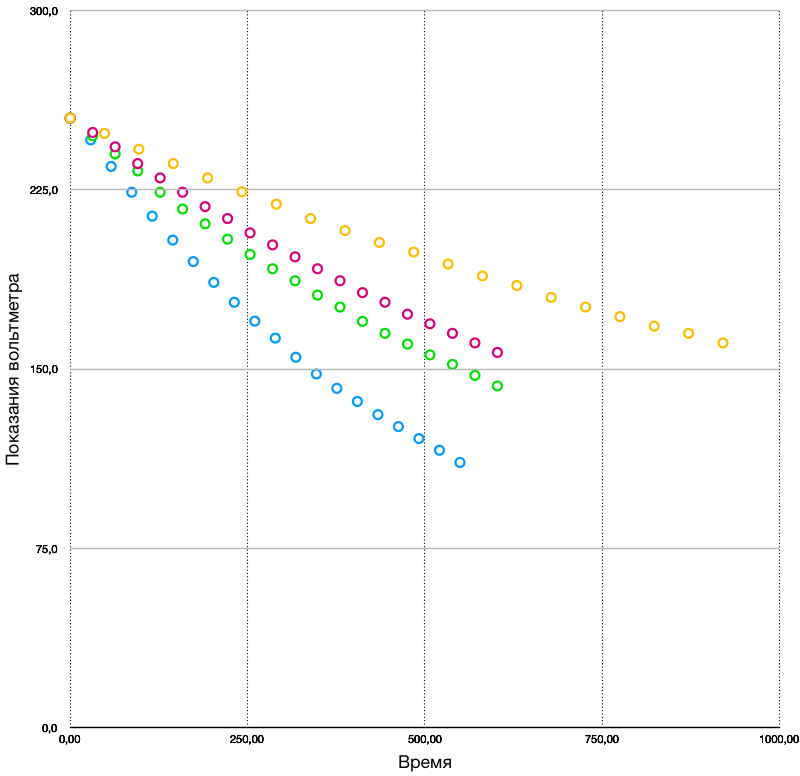
\includegraphics[scale=0.39]{graph1.png} 
        \caption{Зависимость показаний вольтметра от времени при различных давлениях}
        \end{figure}
        \begin{figure}
        \centering
        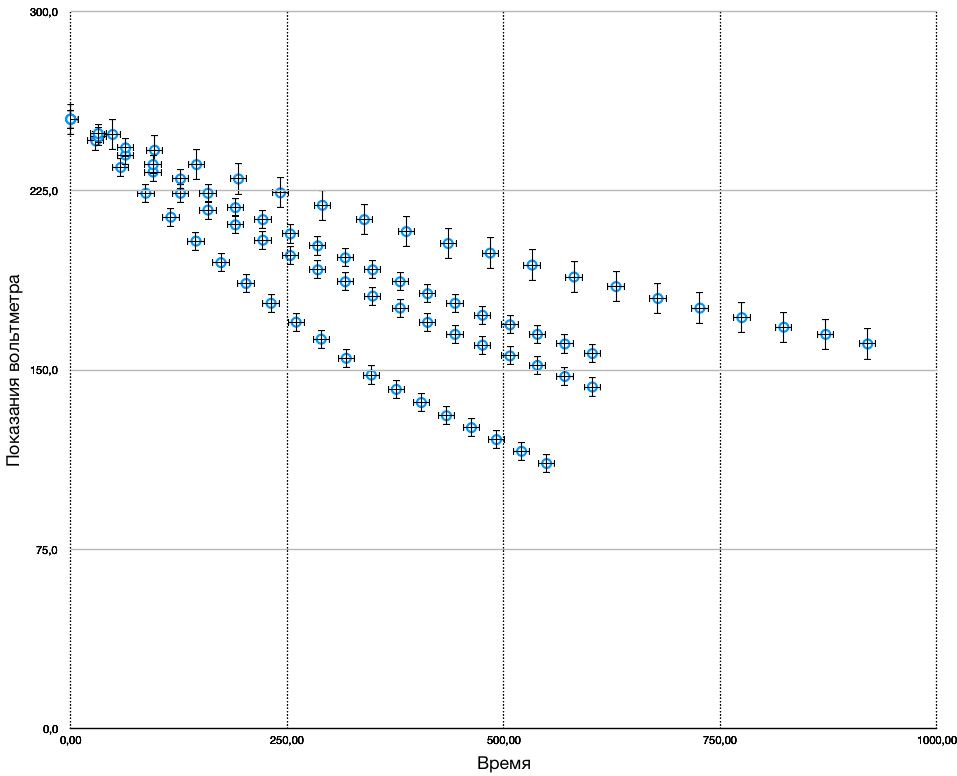
\includegraphics[scale=0.4]{graph3.png} 
        \caption{Зависимость показаний вольтметра от времени при различных давлениях}
        \end{figure}

        Пользуясь формулой 
        \begin{equation}
            D = \dfrac{1}{\tau}\dfrac{VL}{2S}
        \end{equation}
        определим значение коэффициента взаимной диффузии при данном давлении. Запишем результат в таблицу 1.

        Построим график зависимости коэффициента диффузии от величины, обратной давлению, в координатах D(1/P) (\textit{рис. 2}). Убедимся, что данная зависимость линейная. Экстраполируя график к атмосферному (P = 760 Торр) давлению, определим коэффициент взаимной диффузии гелия и воздуха при атмосферном давлении:

        \[ D_\textit{атм} = 225.02/760 + 1.28 \approx 1,58\hspace{3pt} \textit{см}^2/\textit{c} \]
    
        \begin{figure}
        \centering
        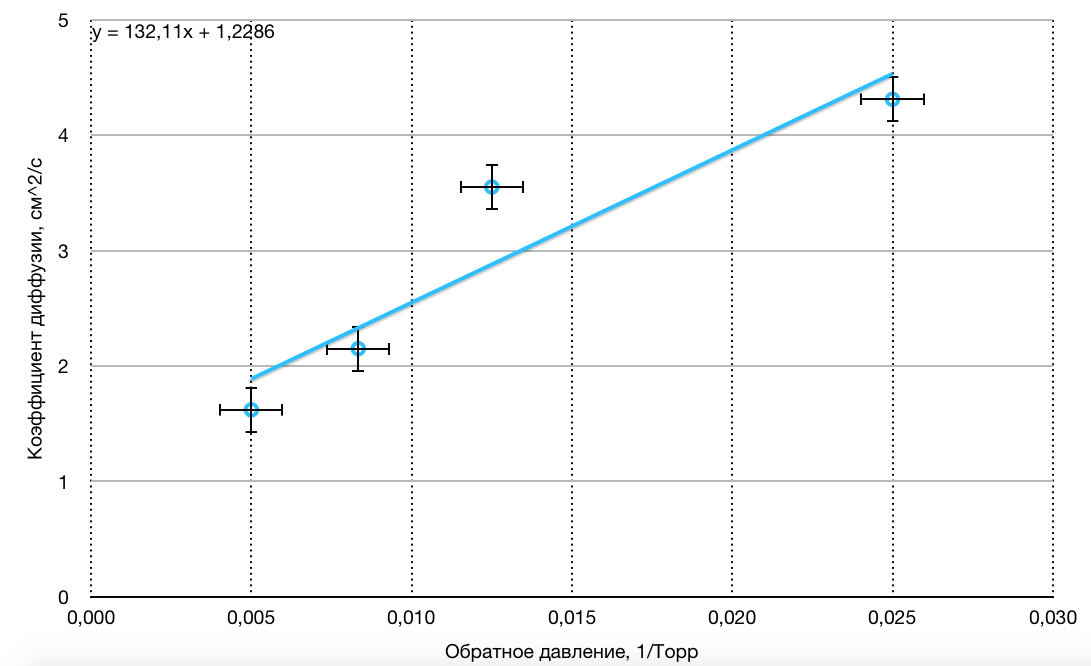
\includegraphics[scale=0.38]{graph2.png} 
        \caption{Зависимость коэффициента диффузии от обратного давления}
        \end{figure}

        Оценим длину свободного пробега и эффективное сечение атомов гелия в условиях эксперимента:
        
        \[D = \frac{1}{3} \overline{v}\lambda = \frac{1}{3} \sqrt{\frac{3RT}{\mu}}\lambda \]
        
        \[\lambda = D\sqrt{\frac{3\mu}{RT}}\]
        
        \[\lambda = \frac{1}{\sqrt{2}\sigma n} \rightarrow \sigma = \frac{kT}{\sqrt{2}\lambda P} \]
        
        Результаты запишем в таблицу 1.
    
\section{Погрешности измерений}
    \begin{table}[!h]
        \begin{center}
            \begin{tabular}{|c|c|c|}
            \hline
            Погрешность величины    & значение      &   причины \\ \hline
            $\sigma (\Delta V)$     &   30 см$^3$   &   данные из установки \\
            $\sigma (\frac{L}{S})$  &   0,5 1/см    &	данные из установки	\\
            $\sigma (\tau)$	        &	0,01 с	    &	точность секундомера в компьютере \\
            $\sigma (T)$            &   1 К         &   точность термометра \\
            $\sigma (D)$	        &	0,05	    &   косвенная погрешность\\	
            \hline
            \end{tabular}
        \caption{ Результаты измерений}
        \end{center}
    \end{table}
    
    \begin{center}
        $\sigma(D) = D \sqrt{(\frac{\sigma(V)}{V})^2 + (\frac{\sigma(\frac{L}{S})}{ \frac{L}{S} })^2 + (\frac{\sigma(\tau)}{\tau})^2}$   
    \end{center}
    
    \begin{center}
        $\sigma(\lambda) = \lambda\sqrt{(\frac{\sigma(D)}{D})^2 + (\frac{\sigma(T)}{T})^2}$
    \end{center}
        
    запишем в таблицу 1.
    \begin{table}[!h]
        \begin{center}
            \begin{tabular}{|c|c|c|c|c|c|c|}
            \hline
            P, торр	&	D см$^2$/c	&	$\Delta D$,  см$^2$/c	&   $\varepsilon D$  &	$\lambda, 10^{-6}$ м	&	$\Delta \lambda$, м	&	$\sigma, 10^{-19}$ м$^2$	 \\
            \hline
            40	&	6,74	&	0,087	&   0,012   &	3,98	&	0,052	&	1,38	\\
            80	&	4,28	&	0,053	&   0,012   &	2,53	&	0,032	&	1,09	\\
            120	&	3,57	&	0,041	&   0,011   &	2,11	&	0,025	&	0,87	\\
            200	&	2,24	&	0,028	&   0.013   &	1,32	&	0,017	&	0,83	\\
            300	&	1,75	&	0,026	&   0,013   &	1,03	&	0,015	&	0,71	\\
            \hline
            \end{tabular}
        \caption{ Результаты измерений}
        \end{center}
    \end{table}
    
    \section{Вывод:}
    
        Мы убедились, что в процессе взаимной диффузии газов зависимость концентрации примеси одного газа в другом зависит от времени экспоненциально. Также экспериментально было установлено, что коэффициент диффузии обратно пропорционален давлению газовой смеси. Коэффициента диффузии при атмосфер- ном давлении: $(6 \pm 0.6) * 10 ^ {-5}$ м2/с.
    
    \section{Приложение: Таблица 2}
        \begin{center}
            \begin{tabular}{ | l | l | l | l | l | l | l | l | l | l |}
                \hline
                P, торр	&	T, c	&   U, мВ	&	$\tau$, c	&	D   &   P, торр	    &   T, c	&	U, мВ	&	$\tau$, c	&	D	\\
                \hline
                40	&	0,00	&	255,0	&	652,6   &	6,74    &   120 &	0,00	&	255,0	&	1233,0	&	3,57	\\
              	    &	28,93	&	245,9	&	  	&	&   &   31,71	&	249,0	&	  	&	\\
              	    &	57,85	&	231,5	&	  	&   &	&   63,41	&	243,0	&	  	&\\
              	    &	86,78	&	224,0	&	  	&	&	&   95,12	&	236,0	&	  	&  	\\
              	    &	112,71	&	217,1	&	  	&	&	&   126,82	&	230,0	&	  	&  	\\
              	    &	144,63	&	204,0	&	  	&	&	&   158,53	&	224,0	&	  	&  	\\
              	    &	173,56	&	195,0	&	  	&	&	&   190,23	&	218,0	&	  	&  	\\
              	    &	202,48	&	186,3	&	  	&	&	&   221,94	&	213,0	&	  	&  	\\
              	    &	231,41	&	178,0	&	  	&	&	&   253,64	&	207,0	&	  	&  	\\
              	    &	260,34	&	170,1	&	  	&	&	&   285,35	&	202,0	&	  	&  	\\
              	    &	289,26	&	163,0	&	  	&	&	&   317,05	&	197,0	&	  	&  	\\
              	    &	318,19	&	155,0	&	  	&	&	&   348,76	&	192,0	&	  	&  	\\
              	    &	347,12	&	148,0	&	  	&	&	&   380,46	&	187,0	&	  	&  	\\
              	    &	376,04	&	142,0	&	  	&	&	&   380,46	&	187,0	&	  	&  	\\
              	    &	404,97	&	136,5	&	  	&	&	&   412,17	&	182,0	&	  	&  	\\
              	    &	433,89	&	131,0	&	  	&	&	&   443,87	&	178,0	&	  	&  	\\
              	    &	462,82	&	126,0	&	  	&	&	&   475,58	&	173,0	&	  	&  	\\
              	    &	491,75	&	121,0	&	  	&	&	&   507,28	&	169,0	&	  	&  	\\
              	    &	520,67	&	116,1	&	  	&	&	&   538,99	&	165,0	&	  	&  	\\
              	    &	549,60	&	111,0	&	  	&	&	&   570,69	&	161,0	&	  	&  	\\
                \hline
                80	&	0,00	&	255,0	&	1028,2	&	4,28    &   200	&	0,00	&	255,0	&	1963,7	&	2,24	\\
              	    &	31,71	&	247,6	&	  	&   &	&   48,44	&	248,6	&	  	&   \\
              	    &	63,41	&	240,0	&	  	&   &   &	96,88	&	242,0	&	  	&	\\
              	    &	95,12	&	232,9	&	  	&   &   &	145,33	&	236,0	&	  	&	\\
              	    &	126,82	&	224,0	&	  	&   &   &	193,77	&	230,0	&	  	&	\\
              	    &	158,53	&	217,0	&	  	&   &   &	242,21	&	224,2	&	  	&	\\
              	    &   190,23	&	210,8	&	  	&   &   &	290,65	&	219,0	&	  	&	\\
              	    &	221,94	&	204,4	&	  	&   &	&   339,09	&	213,0	&	  	&	\\
              	    &	253,64	&	198,0	&	  	&   &   &	387,54	&	208,0	&	  	&	\\
              	    &	285,35	&	192,0	&	  	&   &	&   435,98	&	203,0	&	  	&	\\
              	    &	317,05	&	187,0	&	  	&   &   &	484,42	&	199,0	&	  	&	\\
              	    &	348,76	&	181,0	&	  	&   &   &	532,86	&	194,0	&	  	&	\\
              	    &	380,46	&	176,0	&	  	&   &   &	581,31	&	189,0	&	  	&	\\
              	    &	412,17	&	170,0	&	  	&   &   &	629,75	&	185,0	&	  	&	\\
              	    &	443,87	&	165,0	&	  	&   &   &	678,19	&	180,0	&	  	&	\\
              	    &	475,58	&	160,5	&	  	&   &   &	726,63	&	176,0	&	  	&	\\
              	    &	507,28	&	156,0	&	  	&   &   &	775,07	&	172,0	&	  	&	\\
              	    &	538,99	&	152,0	&	  	&   &   &	823,52	&	168,0	&	  	&	\\
              	    &	570,69	&	147,4	&	  	&   &   &	871,96	&	165,0	&	  	&	\\
              	    &	602,40	&	143,0	&	  	&   &   &	920,40	&	161,0	&	  	&	\\
                \hline
            \end{tabular}
        \end{center}
\end{document}
